\documentclass[border=10pt]{standalone}

\input{../tikz.tex.preamble}
\input{../typography.tex.preamble}

\usetikzlibrary{shapes.geometric, arrows.meta, positioning}

\begin{document}

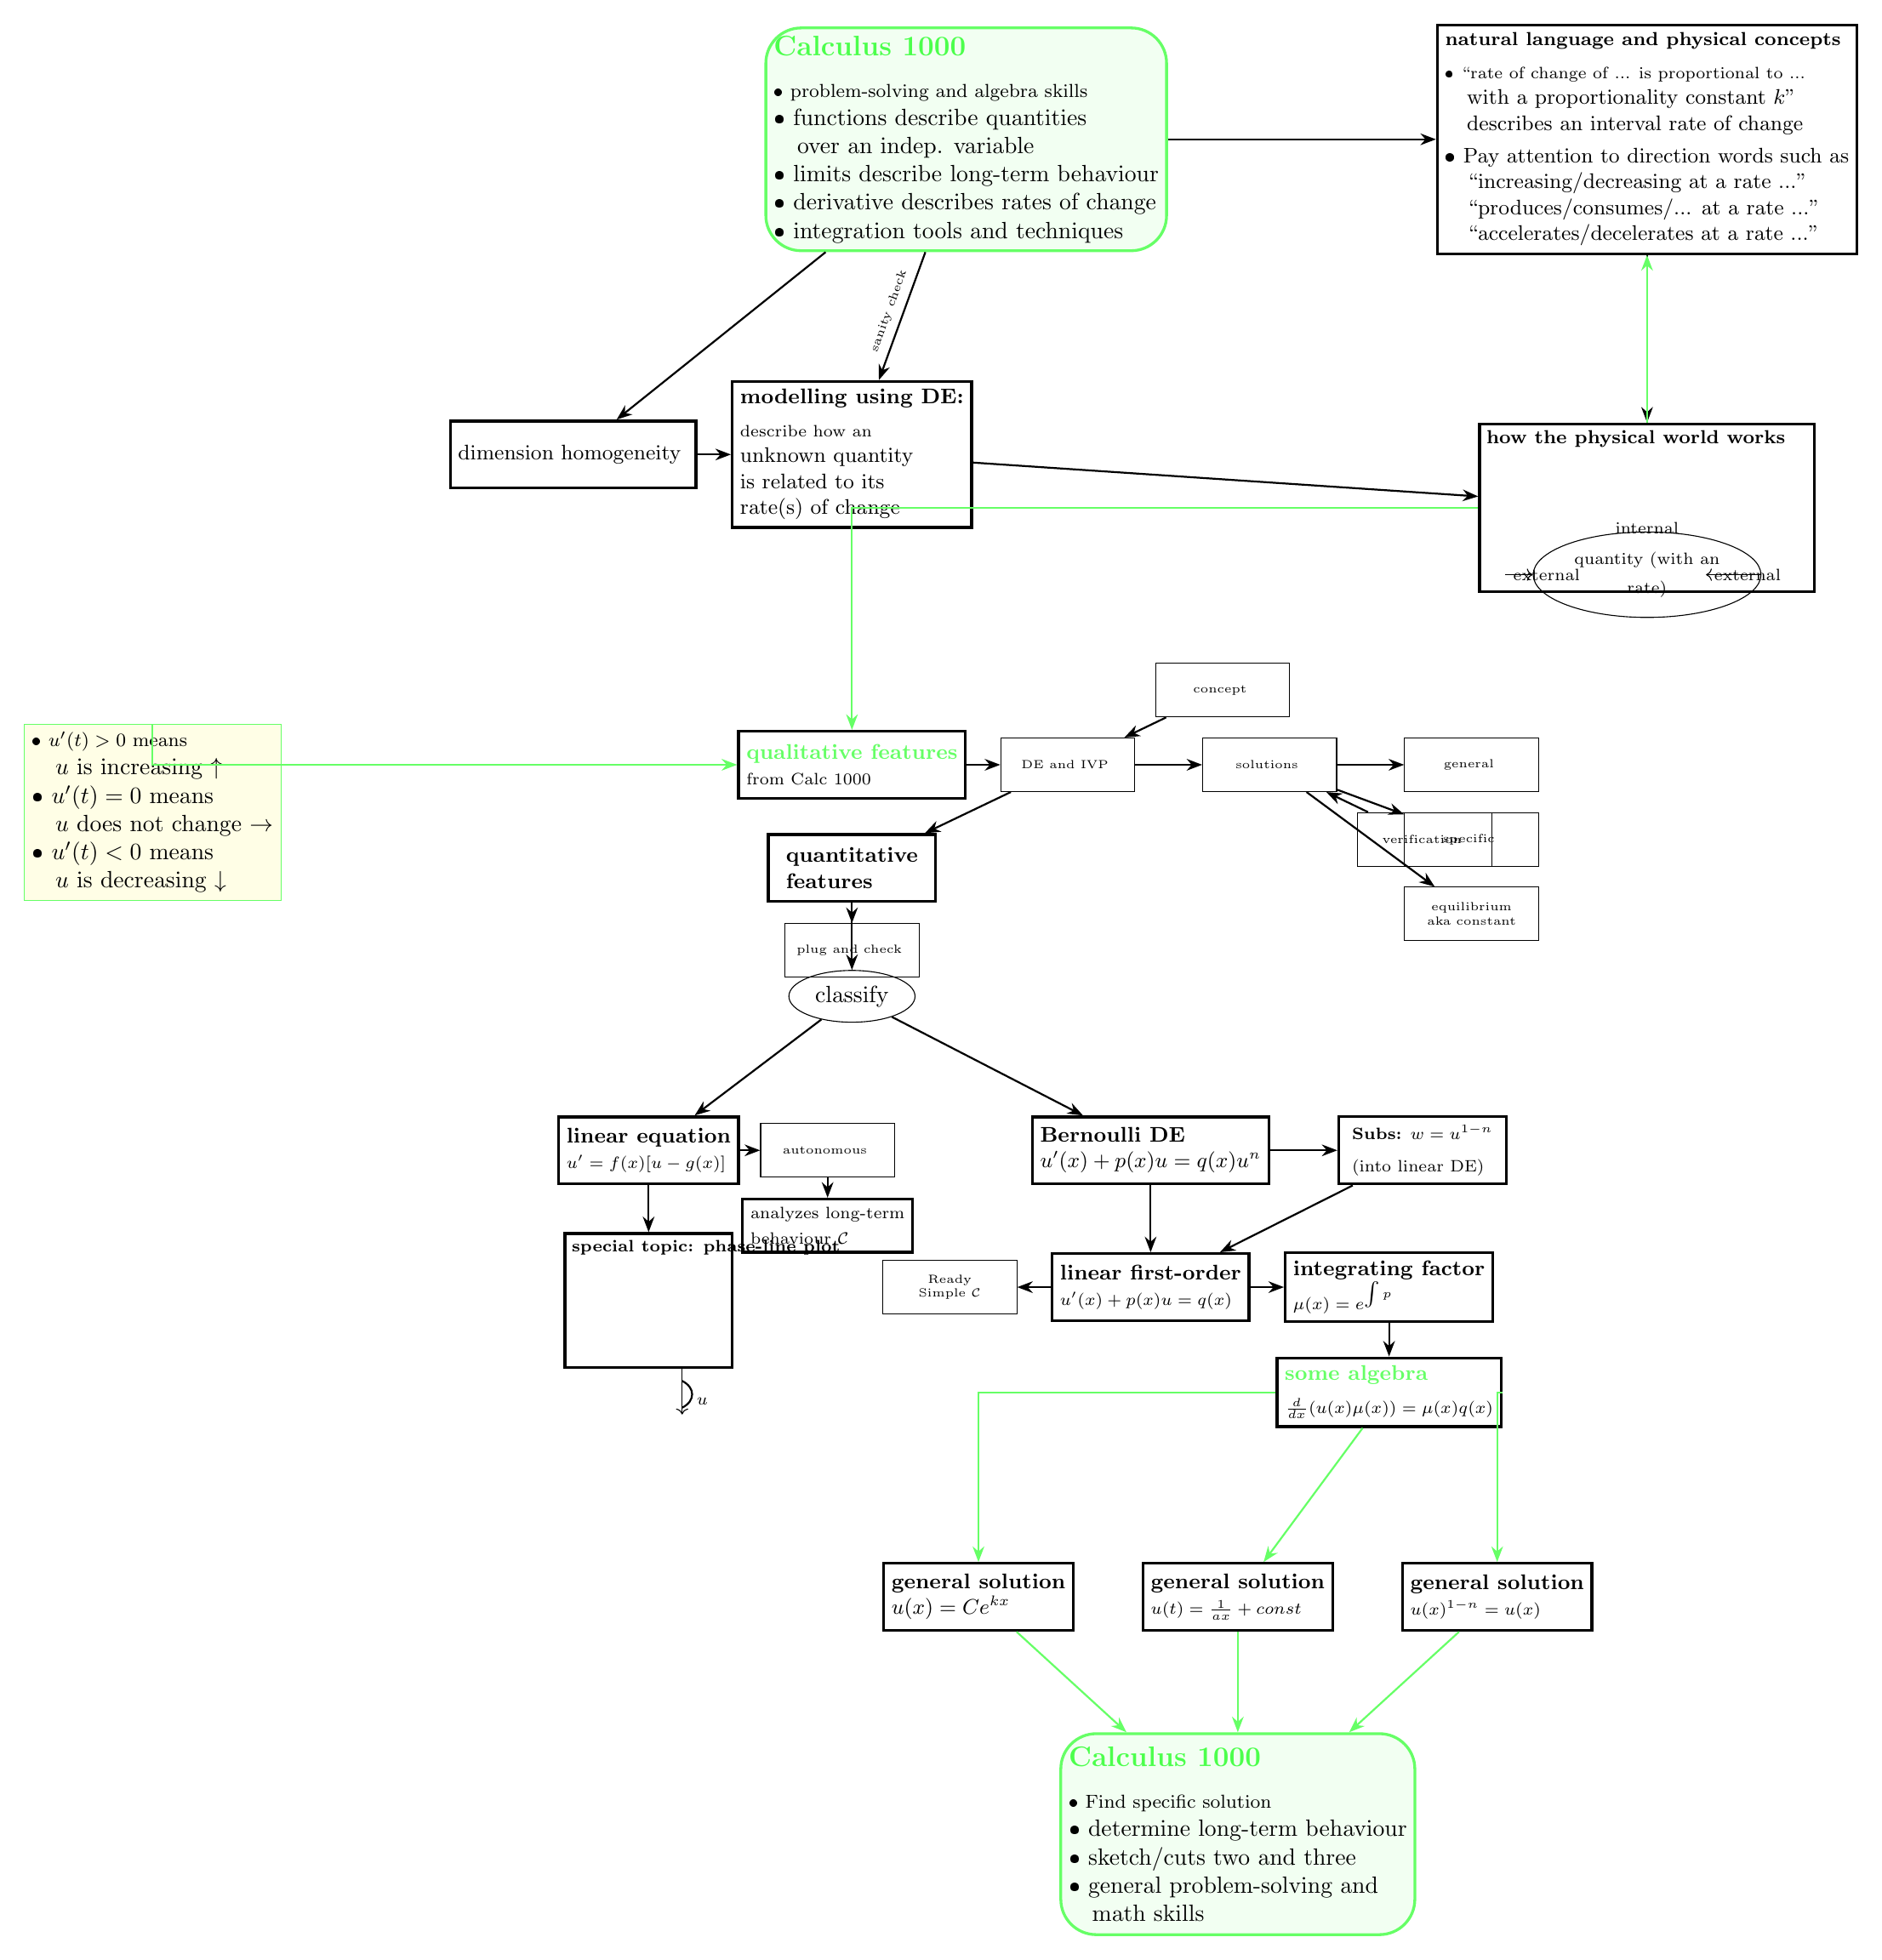
\begin{tikzpicture}[
    node distance=1.5cm and 2cm,
    cloudbox/.style={draw=green!60, fill=green!5, very thick, rectangle, rounded corners=15pt, minimum width=4cm, minimum height=3cm, align=left},
    box/.style={draw=black, very thick, rectangle, minimum width=2.5cm, minimum height=1cm, align=left, font=\small},
    smallbox/.style={draw=black, rectangle, minimum width=2cm, minimum height=0.8cm, align=center, font=\tiny},
    yellowbox/.style={draw=green!60, fill=yellow!10, rectangle, minimum width=2.5cm, align=left},
    arrow/.style={-Stealth, thick},
    greenarrow/.style={-Stealth, thick, green!60},
]

% Top cloud - Calculus 1000 (introduction)
\node[cloudbox] (calc1) at (0,0) {
    \textcolor{green!70}{\large\textbf{Calculus 1000}} \\[0.2cm]
    \footnotesize
    • problem-solving and algebra skills \\
    • functions describe quantities \\
    \quad over an indep. variable \\
    • limits describe long-term behaviour \\
    • derivative describes rates of change \\
    • integration tools and techniques
};

% Natural language box (top right)
\node[box, right=4cm of calc1, minimum width=4.5cm, minimum height=3cm] (natural) {
    \footnotesize \textbf{natural language and physical concepts} \\[0.1cm]
    \scriptsize
    • ``rate of change of ... is proportional to ... \\
    \quad with a proportionality constant $k$'' \\
    \quad describes an interval rate of change \\[0.1cm]
    • Pay attention to direction words such as \\
    \quad ``increasing/decreasing at a rate ...'' \\
    \quad ``produces/consumes/... at a rate ...'' \\
    \quad ``accelerates/decelerates at a rate ...''
};

% Physical world box
\node[box, below=2.5cm of natural, minimum width=5cm, minimum height=2.5cm] (physical) {};
\node[anchor=north west] at (physical.north west) {\footnotesize \textbf{how the physical world works}};

\node (phys-ext1) at ([xshift=-1.5cm, yshift=-1cm]physical.center) {\scriptsize external};
\node[ellipse, draw, align=center] (phys-qty) at ([yshift=-1cm]physical.center) {\scriptsize quantity (with an \\ \scriptsize rate)};
\node (phys-ext2) at ([xshift=1.5cm, yshift=-1cm]physical.center) {\scriptsize external};
\node (phys-int) at ([yshift=-0.3cm]physical.center) {\scriptsize internal};
\draw[->] (phys-ext1) -- (phys-qty);
\draw[->] (phys-qty) -- (phys-ext2);

% Sanity check boxes
\node[box, below left=2.5cm and 1cm of calc1] (sanity1) {
    dimension homogeneity
};

\node[box, right=0.5cm of sanity1, minimum width=3cm] (modelling) {
    \textbf{modelling using DE:} \\[0.1cm]
    \scriptsize describe how an \\
    unknown quantity \\
    is related to its \\
    rate(s) of change
};

% Qualitative features box (left side)
\node[yellowbox, below left=3.5cm and 2.5cm of sanity1] (features) {
    \footnotesize
    • $u'(t)>0$ means \\
    \quad $u$ is increasing $\uparrow$ \\
    • $u'(t)=0$ means \\
    \quad $u$ does not change $\rightarrow$ \\
    • $u'(t)<0$ means \\
    \quad $u$ is decreasing $\downarrow$
};

% Main flow boxes
\node[box, below=3cm of modelling] (qualfeat) {
    \textcolor{green!60}{\textbf{qualitative features}} \\
    \scriptsize from Calc 1000
};

\node[smallbox, right=0.5cm of qualfeat] (de_ivp) {
    DE and IVP
};

\node[smallbox, above right=0.3cm and 0.3cm of de_ivp] (concept) {
    concept
};

\node[smallbox, right=1cm of de_ivp] (solutions) {
    solutions
};

\node[smallbox, below right=0.3cm and 0.3cm of solutions] (verification) {
    verification
};

\node[smallbox, right=1cm of solutions] (general) {
    general
};

\node[smallbox, below=0.3cm of general] (specific) {
    specific
};

\node[smallbox, below=0.3cm of specific] (equilibrium) {
    equilibrium \\
    aka constant
};

\node[box, below=0.5cm of qualfeat] (quant) {
    \textbf{quantitative} \\
    \textbf{features}
};

\node[smallbox, below=0.3cm of quant] (plug) {
    plug and check
};

% Classify node
\node[ellipse, draw, below=1cm of quant] (classify) {
    classify
};

% Bernoulli DE box
\node[box, below right=1.5cm and 2cm of classify] (bernoulli) {
    \textbf{Bernoulli DE} \\
    $u'(x) + p(x)u = q(x)u^n$
};

% Substitution box
\node[box, right=1cm of bernoulli] (sub) {
    \scriptsize \textbf{Subs:} $w = u^{1-n}$ \\[0.1cm]
    \scriptsize (into linear DE)
};

% Linear equation boxes
\node[box, below left=1.5cm and 1cm of classify, minimum width=2cm] (linear) {
    \textbf{linear equation} \\
    \scriptsize $u' = f(x)[u - g(x)]$
};

\node[smallbox, right=0.3cm of linear] (autonomous) {
    autonomous
};

\node[box, below=0.3cm of autonomous, minimum height=0.6cm] (longtime) {
    \scriptsize analyzes long-term \\
    \scriptsize behaviour $\mathcal{C}$
};

% Phase plot box
\node[box, below=0.7cm of linear, minimum width=2.5cm, minimum height=2cm] (phase) {};
\node[anchor=north west] at (phase.north west) {\scriptsize \textbf{special topic: phase-line plot}};
\draw[->] ([xshift=0.5cm, yshift=-1cm]phase.center) -- ([xshift=0.5cm, yshift=-1.7cm]phase.center);
\draw[thick] ([xshift=0.5cm, yshift=-1.2cm]phase.center) .. controls ([xshift=0.7cm, yshift=-1.3cm]phase.center) and ([xshift=0.7cm, yshift=-1.5cm]phase.center) .. ([xshift=0.5cm, yshift=-1.6cm]phase.center);
\node at ([xshift=0.8cm, yshift=-1.5cm]phase.center) {\scriptsize $u$};

% Linear first order box
\node[box, below=1cm of bernoulli] (firstorder) {
    \textbf{linear first-order} \\
    \scriptsize $u'(x) + p(x)u = q(x)$
};

% Homogeneous box
\node[smallbox, left=0.5cm of firstorder] (homosimple) {
    Ready \\
    Simple $\mathcal{C}$
};

\node[box, right=0.5cm of firstorder] (integrating) {
    \textbf{integrating factor} \\
    \scriptsize $\mu(x) = e^{\int p}$
};

% Some algebra box
\node[box, below=0.5cm of integrating, minimum width=3cm] (algebra) {
    \textcolor{green!60}{\textbf{some algebra}} \\[0.1cm]
    \scriptsize $\frac{d}{dx}(u(x)\mu(x)) = \mu(x)q(x)$
};

% General solutions at bottom
\node[box, below left=2cm and 3cm of algebra] (gensol1) {
    \textbf{general solution} \\
    $u(x) = Ce^{kx}$
};

\node[box, right=1cm of gensol1] (gensol2) {
    \textbf{general solution} \\
    \scriptsize $u(t) = \frac{1}{ax} + \text{const}$
};

\node[box, right=1cm of gensol2] (gensol3) {
    \textbf{general solution} \\
    \scriptsize $u(x)^{1-n} = u(x)$
};

% Bottom cloud - Calculus 1000 (outcome)
\node[cloudbox, below=1.5cm of gensol2, minimum width=5cm] (calc2) {
    \textcolor{green!70}{\large\textbf{Calculus 1000}} \\[0.2cm]
    \footnotesize
    • Find specific solution \\
    • determine long-term behaviour \\
    • sketch/cuts two and three \\
    • general problem-solving and \\
    \quad math skills
};

% Arrows from top
\draw[arrow] (calc1) -- (natural);
\draw[arrow] (natural) -- (physical);
\draw[greenarrow] (physical) -- (natural);
\draw[arrow] (calc1) -- node[above, sloped, font=\tiny] {sanity check} (modelling);
\draw[arrow] (calc1) -- (sanity1);
\draw[arrow] (sanity1) -- (modelling);
\draw[arrow] (modelling) -- (physical);
\draw[greenarrow] (physical) -| (qualfeat);

% Middle section arrows
\draw[arrow] (qualfeat) -- (de_ivp);
\draw[arrow] (concept) -- (de_ivp);
\draw[arrow] (de_ivp) -- (solutions);
\draw[arrow] (solutions) -- (general);
\draw[arrow] (solutions) -- (specific);
\draw[arrow] (verification) -- (solutions);
\draw[arrow] (solutions) -- (equilibrium);
\draw[arrow] (de_ivp) -- (quant);
\draw[arrow] (quant) -- (plug);
\draw[arrow] (quant) -- (classify);

% Classification arrows
\draw[arrow] (classify) -- (linear);
\draw[arrow] (classify) -- (bernoulli);
\draw[arrow] (linear) -- (autonomous);
\draw[arrow] (autonomous) -- (longtime);
\draw[arrow] (linear) -- (phase);
\draw[arrow] (bernoulli) -- (sub);
\draw[arrow] (sub) -- (firstorder);
\draw[arrow] (bernoulli) -- (firstorder);
\draw[arrow] (firstorder) -- (homosimple);
\draw[arrow] (firstorder) -- (integrating);
\draw[arrow] (integrating) -- (algebra);

% Bottom arrows
\draw[greenarrow] (algebra) -| (gensol1);
\draw[greenarrow] (algebra) -- (gensol2);
\draw[greenarrow] (algebra) -| (gensol3);
\draw[greenarrow] (gensol1) -- (calc2);
\draw[greenarrow] (gensol2) -- (calc2);
\draw[greenarrow] (gensol3) -- (calc2);

% Side connections
\draw[greenarrow] (features) |- (qualfeat);

\end{tikzpicture}

\end{document}
